% header
\documentclass[doc,12pt]{apa}

	% most commonly used packages
	\usepackage{epsfig}
	\usepackage{bm}
	\usepackage{apacite}
	\usepackage{epstopdf}
	\usepackage{amssymb}
        \usepackage{amsmath}
        \usepackage{calc}
        \usepackage{mathrsfs}
        \usepackage{cleveref}
        \usepackage{mathtools}
        \usepackage{booktabs}

% ---------- watermark -----------
\usepackage[firstpage]{draftwatermark}
\SetWatermarkAngle{0}
\SetWatermarkFontSize{0.25cm}
\SetWatermarkVerCenter{1.15cm}
\SetWatermarkLightness{0.5}
\SetWatermarkHorCenter{14cm}
\SetWatermarkText{\shortstack[l]{
Ransom, K., Perfors, A. and Navarro, D. J. (2016). Leaping to conclusions: \\
Why premise relevance affects argument strength. Cognitive Science, 40, 1775-1796\\
https://doi.org/10.1111/cogs.12308
}}
\SetWatermarkScale{1}
% -------------------------------


	% most commonly used commands
        % \newcommand{\category}[1]{\mbox{\sc #1}}
        \newcommand{\category}[1]{\textsc{#1}}
        \newcommand{\data}{{data}}
 % need vertical bar at end of next line to avoid triggering font lock
 % bug in aquamacs whereby | introduces verbatim section
	\newcommand{\given}{\, | \, } %|
	\newcommand{\TODO}{ {\bf [TODO]} }
        \newcommand{\cbi}{category-based induction}
        \newcommand{\responsedelta}{\Delta S}
        \newcommand{\bigh}{\mathcal{H}}
        \newcommand{\bigx}{\mathscr{X}}
        \newcommand{\bigc}{\mathscr{C}}
        \newcommand{\conc}{\textit{conclusion}}
        \newcommand{\evidence}{x}
        \newcommand{\relevant}{\textsc{Both Relevant}}
%        \newcommand{\relevantdata}{\textsc{No Story$_{\text{relevant fillers}}$}}
        \newcommand{\relevantdata}{\textsc{Relevant Fillers}}
        \newcommand{\randomdata}{\textsc{Random Fillers}}
%        \newcommand{\relevantdata}{\textsc{Neutral Story $+$ Relevant Fillers}}
%        \newcommand{\randomdata}{\textsc{Neutral Story $+$ Random Fillers}}
        \newcommand{\random}{\textsc{Both Random}}
        \newcommand{\neutral}{\textsc{Neutral Story}}
        \newcommand{\weak}{\textsc{Weak}}
        \newcommand{\strong}{\textsc{Strong}}
        %\crefname{equation}{Eqn.}{Eqns.}
        \crefname{equation}{Equation}{Equations}
        %\crefformat{equation}{Eqn.~(#2#1#3)}
        %\Crefformat{equation}{Eqn.~(#2#1#3)}{Eqns.~(#2#1#3)}
        \crefformat{figure}{Figure~#2#1#3}
        \Crefformat{figure}{Figure~#2#1#3}
        \crefformat{table}{Table~#2#1#3}
        \Crefformat{table}{Table~#2#1#3}
        \crefformat{argument}{(#2#1#3)}

        \newcommand{\oneargument}[2]{{#1} $\rightarrow$ {#2}}
        \newcommand{\oneverboseargument}[3]{{#1} $\xrightarrow{\mbox{~\scriptsize{#3}}~}$ {#2}}
        \newcommand{\twoargument}[3]{\{{#1}, {#2}\} $\rightarrow$ {#3}}
        \newcommand{\threeargument}[4]{\{{#1}, {#2}, {#3}\} $\rightarrow$ {#4}}
        \newcommand{\stimtableentry}[6]{{#1} & {#2} &
          \oneargument{\category{#3}}{\category{#4}} & \category{#5} &
          \category{#6} \\ }

%        \newcommand{\monowin}[2]{{#1} : {#2} \scriptsize{($\bm{M_{\mu \geq 0}}$ : $M_{\mu=0}$)}}
%        \newcommand{\monolose}[2]{{#1} : {#2} \scriptsize{($M_{\mu \geq 0}$ : $\bm{M_{\mu=0}}$)}}
%        \newcommand{\nonmonowin}[2]{{#1} : {#2} \scriptsize{($\bm{M_{\mu<0}}$ : $M_{\mu=0}$)}}
%        \newcommand{\nonmonolose}[2]{{#1} : {#2} \scriptsize{($M_{\mu<0}$ : $\bm{M_{\mu=0}}$)}}
%        \newcommand{\nonmonodraw}[2]{{#1} : {#2} \scriptsize{($M_{\mu<0}$ : $M_{\mu=0}$)}}

        \newcommand{\monowin}[2]{{#1} : {#2} \scriptsize{($\bm{\mu > 0}$ : $\mu=0$)}}
        \newcommand{\monolose}[2]{{#1} : {#2} \scriptsize{($\mu > 0$ : $\bm{\mu=0}$)}}
        \newcommand{\nonmonowin}[2]{{#1} : {#2} \scriptsize{($\bm{\mu<0}$ : $\mu=0$)}}
        \newcommand{\nonmonolose}[2]{{#1} : {#2} \scriptsize{($\mu<0$ : $\bm{\mu=0}$)}}
        \newcommand{\nonmonodraw}[2]{{#1} : {#2} \scriptsize{($\mu<0$ : $\mu=0$)}}


% title matter

% Revision
\title{Leaping to conclusions: Why premise relevance affects argument strength}
\author{\normalsize Keith Ransom \\ Amy Perfors \\ Danielle J. Navarro}
\affiliation{School of Psychology \\ University of Adelaide}
\acknowledgements{Correspondence concerning this article should be addressed to Keith Ransom, School of Psychology, University of Adelaide SA 5005, Australia (keith.ransom@adelaide.edu.au). DJN received salary supported from ARC grant FT110100431 and AP from ARC grant DE120102378. Research costs were funded through ARC grant DP110104949.}
\rightheader{Premise Relevance and Argument Strength}
\shorttitle{Premise Relevance and Argument Strength}
\leftheader{Premise Relevance and Argument Strength}

\abstract{%
% Revision
  Everyday reasoning requires more evidence than raw data alone can provide.
%
We explore the idea that people can go beyond this data by reasoning about how the data was sampled. This idea is investigated through an examination of {\em premise non-monotonicity}, in which adding premises to a category-based argument weakens rather than strengthens it.
% Revision
Relevance theories explain this phenomenon in terms of people's sensitivity to the relationships amongst premise items.  We show that a Bayesian model of \cbi\ taking premise sampling assumptions and category similarity into account complements such theories and yields two important predictions: first, that sensitivity to premise relationships can be violated by inducing a weak sampling assumption; and second, that premise monotonicity should be restored as a result.  We test these predictions with an experiment that manipulates people's assumptions in this regard, showing that people draw qualitatively different conclusions in each case.
%
\vskip\belowdisplayskip%
{\bf Keywords}: Bayesian modelling; category-based induction; non-monotonicity; relevance theory; sampling assumptions.
}

% start of document
\begin{document}
\maketitle
\noindent


% start of content
% ------------------------------------------------------------------------
\section{Introduction}
\label{intro}

% Revision
Whereas formal deductive reasoning provides a solid bridge from premise to conclusion, everyday reasoning requires an inferential leap.
%
But what assumptions support such a leap when raw data alone cannot?  This question is relevant to the understanding of \cbi, an important and representative form of inductive reasoning. In a typical \cbi\ task, people are presented with a conclusion supported by one or more premise statements and asked to rate the strength of the inductive argument as a whole. Similarity-based models, which assume that argument strength is assessed on the basis of similarity between premise and conclusion categories, have successfully accounted for many aspects of people's performance in such tasks \cite{Osh90,Slo93}. Yet there are other characteristics of people's reasoning in this regard that are not adequately predicted on the basis of similarity. These characteristics have been explained as emerging from people's sensitivity to the relevance of different
% Revision
premises and the relationships amongst them \cite{MCSH03}.
%

% Revision
In this paper we explain why and when premise relevance should matter.
We argue that people's reasoning is sensitive to premise relationships because they consider the generative process behind the data they observe. If people made no such considerations, and instead assumed that all data consistent with the truth were equally likely to be observed (a so-called {\em weak sampling} assumption), then a perceived relationship amongst premise items should have no effect on argument strength. We demonstrate this by manipulating people's assumptions about premise selection, and observing that people draw qualitatively different conclusions as a result.  Thus, we reproduce an effect of premise relevance on argument strength demonstrated by \citeA{MCSH03} in a scenario where relevance should matter, and fail to observe the effect where it should not. Furthermore, we argue that the notion of {\em cognitive effect}, central to relevance theory explanations of induction, is neatly captured by a Bayesian theory of \cbi\ that naturally incorporates different assumptions about premise sampling, along with the role of category similarity. Our results offer important corroborating evidence for the relevance theory of induction.
%

We first describe the \cbi\ task, with a focus on arguments in which additional premises lead to weaker rather than stronger conclusions (known as {\em premise non-monotonicity}). We then describe a Bayesian analysis of this task which predicts that whether or not people exhibit premise non-monotonicity depends critically on how they assume the premises were generated in the first place. Finally, we present an experiment in which we manipulate these assumptions. As predicted by our model, people's reasoning differs qualitatively as a function of how they think the premises were sampled.

\subsection{Premise monotonicity and non-monotonicity}

In a typical \cbi\ task participants are asked to rate the strength of
inductive arguments like the following:
%
\begin{equation*}
%\label[argument]{Eagle1}
\begin{array}{rl}
\mbox{{\em premise}} & \mbox{\category{Eagles} have more than one fovea per eye.} \\
\hline
\mbox{{\em conclusion}} & \mbox{\category{Hawks} have more than one fovea per eye.}
\end{array}
\end{equation*}
%
Here we use the notation \oneargument{\category{eagles}}{\category{hawks}} to indicate that this problem
asks people to generalize a property from \category{eagles} to \category{hawks}.\footnote{More precisely, we might denote this \oneverboseargument{\category{eagles}}{\category{hawks}}{{\em mult. foveas}} in order to emphasize the property being extended in the argument. For the most part this detail is not needed for our paper.}
Given that \category{eagles} and \category{hawks} are similar, participants might rate this as a moderately strong argument. Adding premises to an argument typically strengthens it, an effect referred to as {\em premise
  monotonicity} \cite{Osh90}. For instance, the argument \twoargument{\category{eagles}}{\category{falcon}}{\category{hawks}}
appears stronger than \oneargument{\category{eagles}}{\category{hawks}}. The additional premise provides evidence that the property of {\em multiple foveae} should be extended to all birds of prey, and is not a property of \category{eagles} alone.

However, systematic violations of premise monotonicity have been observed. For example, \citeA{MCSH03} found that people were less willing to endorse the generalization \threeargument{\category{grizzly bears}}{\category{brown bears}}{\category{polar bears}}{\category{buffalo}} than \oneargument{\category{grizzly bears}}{\category{buffalo}}, despite the former having more premises. This {\em non-monotonicity} effect appears to arise because the multiple premise argument provides strong evidence that the property should be extended to bears only, and so weakens the plausibility that buffaloes share the property. This insight is captured in the relevance theory of induction, which suggests that adding premise categories should weaken an argument if the added categories reinforce a property shared by all of the premise categories but not the conclusion \cite{MCSH03}.

%This seems sensible, but {\em why}? If nothing is known about the way premises are sampled, then a premise should offer equal evidence for any consistent hypothesis; that a premise may seem more relevant to one hypothesis over another should not matter.

%Consider two properties shared by all the premise categories: one that is also shared by the conclusion category and the other that is not. The plausibility that the first property, over the second, represents the appropriate basis for induction should not change when a premise is added; nothing about the additional premise should be informative in this regard.

% Revision
This seems sensible, but {\em why} is it so? If nothing can be assumed about the way premises are sampled, then there is no reason to expect a more relevant premise to be advanced in argument over a less relevant one; the notion that a perceived relationship between premise items represents the appropriate basis for induction, gains no special credence simply by virtue of being put forward.  But in the real world arguments are rarely (if ever) constructed from randomly sampled facts. It makes sense for people to assume that arguments are constructed by sampling relevant facts to support conclusions and achieve communication goals. Wilson and Sperber's account of {\em relevance theory} \cite{WS04} and Grice's {\em co-operative principle} \cite{Gri89}, upon which their theory is based, each offer explanations for why utterances raise an expectation of relevance on the part of the listener. For Grice, the raised expectation comes about because people, for the most part, follow communicative conventions that encourage relevance. But such a heightened expectation should serve only to sharpen the ability to discriminate inputs on the basis of relevance. A reasonable variation in relevance should exist in the first place.

Wilson and Sperber go further than Grice, arguing that neither a communicative convention nor a communicative context are strictly necessary for an enhanced perception of relevance. A tendency to maximize relevance, they contend, is a fundamental feature of our cognitive systems, arising from the need to make the most efficient use of processing resources. To give an example, there are a number of theoretical results showing that positive evidence has stronger evidentiary value than negative evidence under plausible assumptions\footnote{The critical assumption is that we live in a world in which most items do not have most properties. This seems intuitive (e.g., \textsc{foxes} are {\it furry}, but \textsc{fish}, \textsc{fears} and \textsc{footprints} are not), but some care is needed in substantiating the point. From a logical standpoint any ``sparse'' property (possessed by a minority of entities) is mirrored by a ``non-sparse'' complement. However, they need not be equally salient nor equally useful when describing the world: people are more likely to think that {\it furry} (sparse) as a meaningful property than {\it non-furry} (non-sparse). Indeed, what \citeA{NP11} show is that in any world where entities are not completely homogeneous, the categories and properties that intelligent agents attend to should display this sparsity bias.} about the environment \cite<e.g.,>{KH87,NP11}. Given this, maximizing relevance should lead people to prefer to give and to receive positive evidence, and will therefore treat positive premises (of the form ``item $x$ has property $p$'') as more  relevant than negative ones.

%At the very least, we can say that people communicate about items having a property by generating examples of things with that property rather than without it; this has been shown to be informationally optimal in a variety of circumstances \cite<e.g.,>{KH87,NP11}.

%If people assume premises are selected for a communicative purpose (or at the very least strongly sampled) then a relationship amongst premise categories should affect argument strength.

% Revision
If people assume premises are sampled based on relevance then any property shared by the premises will gain plausibility as the correct basis for induction and stronger inferences to that effect should result.
For example, if I want to convey the range of animals that share a particular property, and I want to be as relevant as possible, then I should select additional examples that best capture the appropriate range. Returning to the bears example, had I wanted to convey the message that many species had some property, not just bears, you might reasonably have expected me to mention a different kind of animal. So my choosing further examples of bears when extending my argument provides evidence that only bears have the property. Qualitatively, this reasoning explains why people exhibit premise non-monotonicity in this situation. This intuition can be reinforced quantitatively by the mathematics of Bayesian probability theory, as we explain in the next section.

\subsection{A model for reasoning in category-based induction}

Consider a standard Bayesian approach to \cbi\ tasks \cite{Hei98,ST03}. Suppose the learner is given a one premise argument of the form \oneverboseargument{$x$}{$y$}{$p$}. Let $h$ denote one possible hypothesis about how far property $p$ should be extended, and $P(h)$ denote the reasoner's prior bias to think that $h$ describes the true extension of property $p$. Having observed that item $x$ possesses property $p$, the posterior degree of belief in $h$ is given by Bayes' rule:
\begin{equation}
\label{eqn:bayes}
P(h \given x) = \frac{ P(x \given h ) P( h ) }{ \sum_{h^\prime} P(x \given h^\prime ) P( h^\prime ) }.
\end{equation}
Here, $P(x \given h)$ is the likelihood, which specifies the probability that the argument would have used $x$ as a premise if $h$ were the true extension of property $p$.
The sum in the denominator is taken over all hypotheses that the reasoner might consider regarding the extension of property $p$. When an argument contains multiple premise items $x_1,\ldots,x_k$, the likelihood is given by the product of each of the individual probabilities, $\prod_{i=1}^k P(x_i \given h )$.
% For now, we have agreed to skip over this independence assumption]}.
% Revision: TODO: Should we revisit this independence assumption - it feels  more dubious now that we are talking about premises being sampled such that a relationship between them is highlighted.
In order to evaluate the claim that item $y$ also possesses property $p$, a  Bayesian reasoner sums the posterior probabilities of all hypotheses that are consistent with the claim. Thus, the argument strength is given by:
\begin{equation}
P( y \given x ) = \sum_{h : y \in h} P(h \given x).
\end{equation}
This model has two components, the prior $P(h)$ and the likelihood $P(x|h)$.  In our application of the model, the prior reflects the similarity amongst premise categories. As described in Appendix A, we use empirical similarity data to set $P(h)$ and simulations to check that the qualitatively important effects are not overly sensitive to the particular data collected.

The likelihood is critical to an understanding of when and why premise relevance matters: it naturally captures different assumptions people may make about how the premises were generated. For instance, a naive reasoner might assume that the premise items for an argument are selected at random from the set of true facts about the property $p$. This is called {\em weak sampling}.
Since the item $x$ is chosen randomly, weak sampling allows premises to present negative evidence (i.e.,``item $x$ does not have property $p$'').
For a premise presenting evidence that item $x$ has property $p$, the weak sampling likelihood function is:
\begin{equation}
\label{eqn:weaksampling}
P(x \given h) \propto \left\{
  \begin{array}{l l}
    1 & \quad \textrm{if $x \in h$} \\
    0 & \quad \textrm{otherwise}
  \end{array} \right.
\end{equation}
In essence, when presented with item $x$, a learner assuming weak sampling falsifies all hypotheses inconsistent with the premise but does not alter their beliefs in any other respect -- the fact that $x$ was chosen over other items has no additional relevance to the reasoning problem. As a result, such a learner will be less likely to demonstrate premise non-monotonicity. If premises are generated randomly, seeing \category{black bears} in addition to \category{grizzly bears} does not act as a ``hint'' that only bears have the property in question. Rather, because there are almost no hypotheses that could be falsified by the additional \category{black bears} premise that were not already falsified by the \category{grizzly bears} premise, the additional information is largely irrelevant.

The simplicity of the weak sampling model and its connection to falsification is appealing. However, as we have seen, it provides a poor description of how
inductive arguments are constructed in everyday reasoning. If a learner expects an argument to be constructed using positive examples, then a weak sampling assumption is no longer tenable. A simple alternative is {\em strong sampling} \cite{TG01,ST03}, in which a premise item is selected {\it only} from those exemplars that possess property $p$. As noted earlier, this restriction makes sense if people expect to receive relevant evidence.
%\footnote{The strong sampling model is not intended to capture all the complexity of everyday inferences. For instance, if the learner expects {\em mostly} positive evidence, a mixed sampling model can be used \cite{NDL12}. Richer pragmatic assumptions can be captured using pedagogical sampling models \cite{SGG14}. Neither complication is necessary in the current context.}
This gives the likelihood function
\begin{equation}
\label{eqn:strongsampling}
P(x \given h) = \left\{
  \begin{array}{l l}
    \frac{1}{|h|} & \quad \textrm{if $x \in h$} \\
    0 & \quad \textrm{otherwise}
  \end{array} \right.
\end{equation}
where $|h|$ denotes the {\em size} of hypothesis $h$. In this context, the size is calculated by counting the number of items that possess property $p$ assuming hypothesis $h$ is true.

Under strong sampling, the item presented has relevance beyond falsification. That is, a premise provides more evidence for a small hypothesis than it does for a larger one \cite{TG01}. A learner who sees multiple premise items consistent with one small hypothesis will come to prefer that hypothesis over other, broader hypotheses, even when the broader hypothesis happened to be originally preferred.  As noted in previous research \cite{Fer06,KT09,VMS13}, this phenomenon provides a potential explanation for why people sometimes exhibit premise monotonicity and at other times non-monotonicity.

Compare the one premise argument \oneargument{\category{chimpanzees}}{\category{gorillas}} to the two premise argument \twoargument{\category{chimpanzees}}{\category{orangutan}}{\category{gorillas}}. Both premises are consistent with a small hypothesis (i.e., that all primates have that property). Because gorillas are also primates the additional evidence provided by the \category{orangutan} premise acts to strengthen the argument: premise monotonicity is satisfied.  In contrast, compare the one premise argument \oneargument{\category{grizzly bears}}{\category{lion}} to the two premise argument \twoargument{\category{grizzly bears}}{\category{black bears}}{\category{lion}}. In the one premise variant, the reasoner might reasonably believe that the property extends to all mammals or all predators, and so there is at least some chance that \category{lions} possess the property. However, when \category{black bears} is added to the list of premise items, the reasoner has strong evidence in favor of a small hypothesis, namely that the property is common only to bears. This produces a non-monotonicity effect, since an additional positive observation acts to weaken the conclusion.

Importantly, this explanation relies on the assumption of strong sampling. It is this assumption that gives a premise item relevance over and above its use for falsification. In the bears example above, the effect occurs because a second bear premise provides strong evidence for the (smaller) ``bears'' hypothesis relative to the  (larger) ``all predators'' and ``all mammals'' hypotheses, even though all three are consistent with both premises. Under a weak sampling assumption, premise items have no relevance beyond falsification, and this shift does not occur.

% Revision
If strong sampling represents an assumption that premise selection is biased towards relevant items%
\footnote{The strong sampling model is not intended to capture all the complexity of selecting items for relevance. For instance, richer pragmatic assumptions can be captured using pedagogical sampling models \cite{SGG14}. This complication is not necessary in the current context but some implications are addressed in more detail in the discussion.}
and weak sampling represents the assumption that is is not, then it is reasonable to consider that the bias to expect relevant premises might vary not just in kind, but also in degree. A {\it mixed sampling} model can be used to capture this situation in a straightforward way \cite{NDL12}. Under mixed sampling, the likelihood function becomes:
\begin{equation}
\label{eqn:mixedsampling}
P(x \given h) = \left\{
  \begin{array}{l l}
    \theta \frac{1}{|h|} + (1 - \theta) \frac{1}{|\bigx|} & \quad \textrm{if $x \in h$} \\
    0 & \quad \textrm{otherwise}
  \end{array} \right.
\end{equation}
where $|\bigx|$ represents the number of possible premise items, and $\theta$ represents the probability that the premise item $x$ was strongly sampled. When $\theta=0$ the model is equivalent to weak sampling and has no bias towards positive evidence. In contrast, when $\theta=1$ the bias is so extreme that the learner believes it is impossible to receive negative evidence, and the mixed sampling model becomes equivalent to strong sampling.

The notion that people are sensitive to how the premises were generated represents an intriguing and testable prediction.
% Revision
If reasoners have an expectation of premise relevance and thus expect premises to be biased towards positive evidence, they should show premise non-monotonicity for the bears example.
%
If, on the other hand, they assume that premise items have been selected at random (i.e., weakly sampled), then premise monotonicity should be exhibited. Note that this prediction stands in contrast to the predictions of similarity based models \cite{Osh90,Slo93} neither of which incorporate any sensitivity to the mechanism by which the premises are generated. To that end, we present experimental evidence that premise monotonicity can be systematically manipulated by changing the assumptions people make about the origins of the data. Not only do we see qualitative reversals from monotonic to non-monotonic reasoning consistent with a change from weak to strong sampling, we also find that the transition occurs in a graded fashion consistent with the smoothly varying bias parameter in the mixed sampling model.

\section{Experiment}

%The experiment takes the form of a category based induction task in which we use a cover story and filler trials to reinforce a particular sampling assumption. In the $\relevant$ condition, people are told that the premises have been given to them by a helpful confederate, and the filler items used support this impression; in the $\random$ condition they are persuaded that the premises are generated randomly. We also employ a neutral cover story in two further conditions: the $\relevantdata$ condition which uses the same filler items as the $\relevant$ condition, and $\randomdata$ whose fillers match the $\random$ condition. %As predicted, people show premise non-monotonicity in the $\relevant$ condition, but not the $\random$ condition, whilst the results of the two neutral conditions appear consistent with a mixed sampling assumption. These results are captured by the Bayesian model described above.

\subsection{Method}

\subsubsection{Participants}

%295 adults were recruited via Amazon Mechanical Turk, and were each paid \$0.50
%(USD) for the 5-10 minutes participation. 29 were excluded due to
%browser incompatibility, and the remaining 266  were aged 18 to
%69 years (median age 27, 69\% male).
%253 participants were in the United States, with 13 located elsewhere.

% Revision
590 adults were recruited via Amazon Mechanical Turk, and were each paid \$0.50 (USD) for the 5--10 minutes participation. 52 were excluded due to
browser incompatibility, and the remaining 538 were aged 18 to
69 years (median age 28, 65\% male).
500 participants were in the United States, with 38 located elsewhere.

\subsubsection{Procedure}

\begin{figure}[t]
\begin{center}
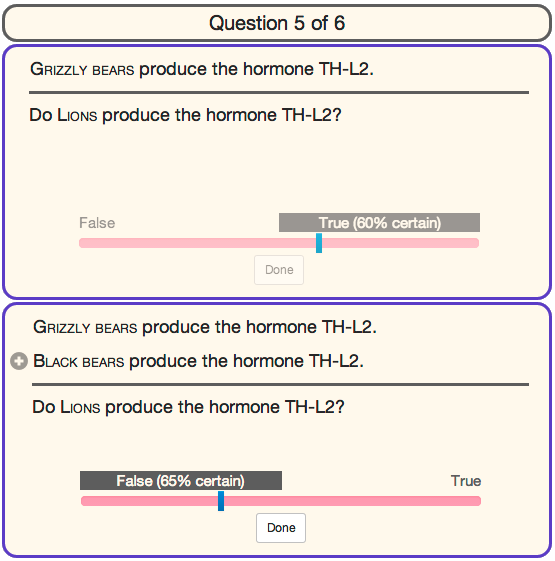
\epsfig{file=Q5.png,width=8cm}
\vspace{-3mm}
\caption{%
An illustration of the on-screen presentation of a trial shown at the
point where the second premise has been revealed. The one premise argument
is displayed on the upper portion of the display, while the two premise form is on the lower portion. The rectangular ``slider'' (disabled on
the upper portion, enabled in the lower) allows participants to respond
``True'' or ``False'' and indicate the level of certainty in their response.
}
\label{fig:trial}
\end{center}
\end{figure}

A cover story informed people that they would be making judgments concerning well established facts about the properties of animals. Each trial began by presenting a fact about one animal and then asking about a second. For example, they might first be told that grizzly bears produce the hormone TH-L2, and then asked whether lions also produce TH-L2. Responses were collected using a slider bar that allowed people to produce answers ranging from ``100\% false'' to ``100\% true'', as shown in \cref{fig:trial}. They were then told about a second animal, and asked to revise their original judgment by moving a different slider. The dependent measure for each trial is the difference between these two judgments. If the endorsement of the conclusion is stronger on the second occasion, premise monotonicity is satisfied. If the difference is negative, non-monotonicity is observed.

\subsubsection{Conditions}

%Participants were randomly assigned to one of two conditions, each involving a cover story designed to encourage a particular sampling assumption about how the second fact was generated. In the \relevant\ condition participants were told that the extra facts were provided by past players of the game who were trying to select a helpful example of an animal with the property in question.  The story was designed to promote the idea that facts were generated with intent, similar to strong sampling or pedagogical sampling. In the \random\ condition people were told that they would select a card from a deck displayed face down on-screen. This card would disclose whether or not a particular animal had the property in question. In contrast to the \relevant\ story, this story was designed to support the assumption of weak sampling by encouraging the belief that facts were being sampled at random.

% Revision
Participants were randomly assigned to one of the four conditions, each involving a different combination of cover story and filler trials. The cover story informed people about how the second fact in each trial was generated, while the filler trials were designed to be consistent with either a strong or weak sampling assumption. In the \relevant\ condition, participants were told that the extra facts were provided by past players of the game who were trying to select a helpful example of an animal with the property in question. The story and the filler trials were designed to promote the idea that facts were chosen on the basis of relevance, similar to strong sampling. In the \random\ condition people were told that they would select a card from a deck displayed face down on-screen. This card would disclose whether or not a particular animal had the property in question. In contrast to the \relevant\ condition, the story and filler items were designed to support the assumption of weak sampling by encouraging the belief that facts were being sampled at random. To allow us to investigate whether the premises alone had an effect on sampling assumptions we ran two further experimental conditions.  The \relevantdata\ condition employed a neutral cover story giving no information about how the premises were selected, and used the same filler items as the \relevant\ condition. Likewise, the \randomdata\ condition employed a neutral cover story, but used the same filler items as the \random\ condition.

\subsubsection{Stimuli}

\begin{table}[t]
\hspace{-5mm}
\scriptsize
\begin{tabular}{rllll}
\toprule
 & & & \multicolumn{2}{c}{Additional example} \\
\cmidrule{4-5}
 Trial & Property to be generalized & First generalization & \textsc{Relevant} & \textsc{Random} \\
\midrule
\stimtableentry{Filler 1}{have more than one fovea per eye}{eagles}{doves}{+hawks}{$-$tortoises}
\stimtableentry{Filler 2}{have mammary glands}{elephants}{deers}{+cows}{+anteaters}
\stimtableentry{Target 1}{have a bite force greater than 500 BFU}{tigers}{ferrets}{+lions}{+lions}
\stimtableentry{Filler 3}{give birth to underdeveloped
  young}{kangaroos}{wombats}{+koalas}{$-$flamingos}
\stimtableentry{Target 2}{produce the hormone TH-L2}{grizzly
  bears}{lions}{+black bears}{+black bears}
\stimtableentry{Control}{require cystocholamine for brain
  function}{orangutans}{gorillas}{+chimpanzees}{+chimpanzees}
  \bottomrule
\end{tabular}
\vspace{-5mm}
\caption{%
  The property to be generalized, the first generalization, and additional
  example used in the \relevant/\relevantdata\ conditions, and in the \random/\randomdata\ condition. Trials are shown are shown in the order presented in the experiment. All conditions have the same arguments in the key trials ({\bf Target 1}, {\bf Target 2}, and {\bf Control}), differing only in cover story and supporting filler trials. The second generalization that people were required to make is formed by combining the first generalization with the additional example. For example, the second generalization for {\bf Target 1} becomes  \twoargument{\category{tigers}}{\category{+lions}}{\category{ferrets}}.
The ``$-$'' symbol is used to indicate that the statement should be negated: e.g., ``\category{tortoises} {\em don't have} more than one fovea per eye."
}

\label{tbl:stimuli}
\end{table}

All participants were presented with six trials in a fixed order,\footnote{Randomization of trial order would not have made sense in this context. Because the filler items were an important part of the experimental manipulation, it was critical that at least some of these precede the target items; because we did not want the design to be too obvious, we also wanted to include at least one filler in between the two targets.%
%Regardless, since the order was the same in all conditions it is unlikely that the ordering led to any differences between conditions.
} as shown in \cref{tbl:stimuli}. Three of these were especially key and appeared in all conditions. There were two target arguments structured so that they should elicit non-monotonic responding under a strong sampling assumption ({\bf Target 1}: \twoargument{\category{tigers}}{\category{lions}}{\category{ferrets}}; {\bf Target 2}: \twoargument{\category{grizzly bears}}{\category{black bears}}{\category{lions}}). There was also a {\bf Control} argument designed to elicit monotonic reasoning under any mixture of weak or strong sampling (\twoargument{\category{chimpanzee}}{\category{orangutan}}{\category{gorilla}}).% Revision
Finally, each person saw three {\bf Filler} trials, designed to reinforce a particular sampling assumption.  Consistent with strong sampling, the filler trials in the \relevant\ and \relevantdata\ conditions consisted solely of positive examples. In contrast, the filler trials in the \random\ and \randomdata\ conditions included negative examples as well, and appeared much more random.

\section{Results}

\subsection{Model predictions}

%The Bayesian model described above was used to quantitatively predict how a reasoner assuming either weak or strong sampling would reason about the two {\bf Target} arguments and the {\bf Control} argument
%(by setting $\theta=0$ for weak sampling and $\theta=1$ for strong).

The Bayesian model of strong and weak sampling described in \crefrange{eqn:bayes}{eqn:strongsampling} was used to quantitatively predict how a reasoner holding either assumption would reason about the two {\bf Target} arguments and the {\bf Control} argument. In order to extract these predictions, it was necessary to specify a hypothesis space $\bigh$ and a prior distribution $P(\bigh)$.  The hypothesis space simply consisted of all possible sets of the 14 animals common to the two experimental conditions. In order to estimate the prior, we collected similarity ratings for all pairs of the 14 animals. The estimation procedure was an adaptation of the additive clustering technique (\citeNP{SA79}; see also \citeNP{Lee02}, \citeNP{NG08}) and is discussed in more detail in Appendix A.
%
\begin{figure}[t]
\begin{center}
%\begin{tabular}{cc}
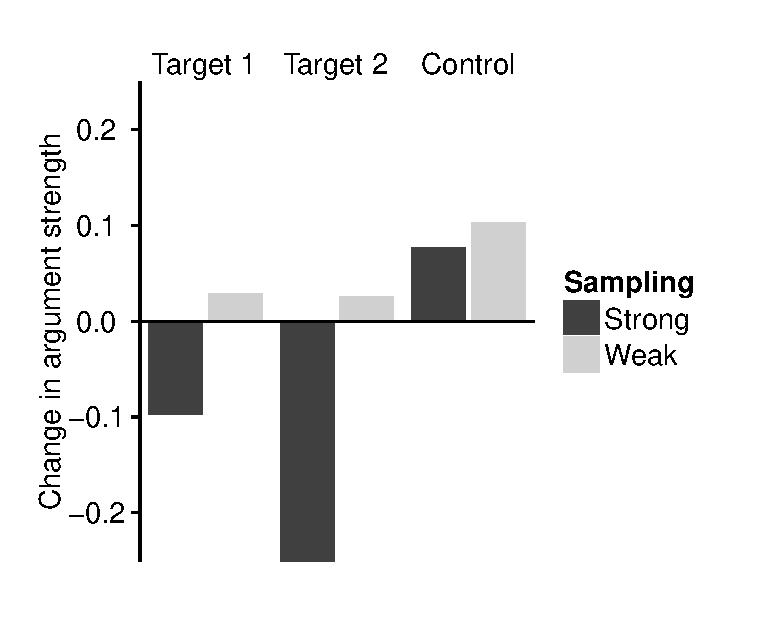
\includegraphics[scale=0.60]{predictions.eps}
%\multicolumn{1}{c}{\small (a) Model predictions} &
%\multicolumn{1}{c}{\small (b) Human performance}
%\end{tabular}
\end{center}
\vspace{-5mm}
\caption{%
  Model predictions for the change in argument strength when an additional premise is introduced (i.e., $P(y|x_1,x_2)-P(y|x_1)$).
  A positive change indicates premise monotonicity, a negative change, non-monotonicity.
  In the {\bf Control} argument, monotonicity is predicted regardless of sampling assumption. For
  both {\bf Target} arguments, a reversal is predicted: premise non-monotonicity is
  expected only under an assumption of strong sampling. (The difference in the magnitude of the predictions between the two {\bf Target} conditions emerges due to the structure of people's real-world
  knowledge about the domain as reflected in the prior, and is incidental to our main point.) %It is unimportant to our main point, which focuses on the qualitative difference between the {\bf Target} and {\bf Control} arguments.
}
\label{fig:predictions}
\end{figure}

\Cref{fig:predictions} shows the resulting model behavior. As predicted previously, when weak sampling is assumed the model indicates premise monotonicity for both {\bf Target} and {\bf Control} trials. Conversely, under strong sampling it predicts non-monotonicity for {\bf Target} trials and monotonicity for {\bf Control} trials. Importantly, while the precise numerical prediction shown in \Cref{fig:predictions} depends on the way in which the prior was derived, the qualitative effect of sampling assumptions is robust with regard to change in details: as discussed in Appendix A, the Bayesian model predicts a shift towards non-monotonicity under strong sampling provided that the prior distribution reflects the conceptual structure of the animal domain.

\subsection{Experimental results}

\begin{table}[t]
\hspace{-5mm}
%\scriptsize
\small
\begin{tabular}{rrrrrrrr}
\toprule
 & & \multicolumn{6}{c}{Argument strength} \\
\cmidrule{3-8}
 & & \multicolumn{2}{c}{Original} & \multicolumn{2}{c}{Revised} & \multicolumn{2}{c}{Change} \\
\cmidrule{3-4} \cmidrule{5-6} \cmidrule{7-8}
 Condition & N & Mean & SE & Mean & SE & Mean & SE \\
\midrule
\multicolumn{2}{c}{\bf Target 1} \\
\relevant & 135 & .283 & .021 & .210 & .021 & -.073 & .013 \\
\relevantdata & 134 & .313 & .023 & .259 & .022 & -.054 & .015 \\
\randomdata & 138 & .301 & .020 & .275 & .020 & -.026 & .014 \\
\random & 131 & .277 & .022 & .307 & .026 & .031 & .021 \\
\multicolumn{2}{c}{\bf Target 2} \\
\relevant & 135 & .523 & .015 & .444 & .023 & -.079 & .023 \\
\relevantdata & 134 & .538 & .017 & .484 & .022 & -.054 & .015 \\
\randomdata & 138 & .534 & .017 & .521 & .020 & -.012 & .014 \\
\random & 131 & .578 & .018 & .616 & .021 & .038 & .013 \\
\multicolumn{2}{c}{\bf Control} \\
\relevant & 135 & .773 & .015 & .863 & .014 & .090 & .013 \\
\relevantdata & 134 & .765 & .015 & .860 & .013 & .096 & .009 \\
\randomdata & 138 & .759 & .013 & .853 & .013 & .093 & .011 \\
\random & 131 & .790 & .016 & .902 & .010 & .111 & .013 \\
% \multicolumn{2}{c}{\bf Target 1} \\
% \relevant & 135 & -.217 & .021 & -.290 & .021 & -.073 & .013 \\
% \relevantdata & 134 & -.187 & .023 & -.241 & .022 & -.054 & .015 \\
% \randomdata & 138 & -.199 & .020 & -.225 & .020 & -.026 & .014 \\
% \random  & 131 & -.223 & .022 & -.193 & .026 & .031 & .021 \\
% \multicolumn{2}{c}{\bf Target 2} \\
% \relevant & 135 &  .023 & .015 & -.056 & .023 & -.079 & .023 \\
% \relevantdata & 134 & .038 & .017 & -.016 & .022 & -.054 & .015 \\
% \randomdata & 138 & .034 & .017 & .021 & .020 & -.012 & .014 \\
% \random  & 131 &  .078 & .018 &  .116 & .021 &  .038 & .013 \\
% \multicolumn{2}{c}{\bf Control Trial} \\
% \relevant & 135 &  .273 & .015 &  .363 & .014 &  .090 & .013 \\
% \relevantdata & 134 & .265 & .015 & .360 & .013 & .096 & .009 \\
% \randomdata & 138 & .259 & .013 & .353 & .013 & .093 & .011 \\
% \random  & 131 &  .290 & .016 &  .402 & .010 &  .111 & .013 \\
\bottomrule
\end{tabular}
\vspace{-5mm}
\caption{%
Mean argument strength ratings (linearly scaled to the range 0 to 1) for the original judgment (after seeing the first premise only), the revised judgment (after seeing the second premise), and mean change in argument strength (the revised rating minus the original rating, linearly scaled to the range -1 to 1), summarised by condition and trial type.
}
\label{tbl:descriptives}
\end{table}

For each trial, participants rated the strength of an argument in a one- and two-premise form. The main question of interest was whether sampling assumptions had an impact upon the way people assessed the evidentiary value of the additional premise. The dependent measure was therefore the response change between the two judgments: a positive response change reflects premise monotonicity, while a negative one reflects non-monotonicity.
% Revision
\Cref{tbl:descriptives} presents mean argument strength ratings based on the one- and two-premise forms, as well as the mean change between judgments, by trial type and condition.

% %
% \begin{figure}[t]
% \begin{center}
% \begin{tabular}{cc}
% %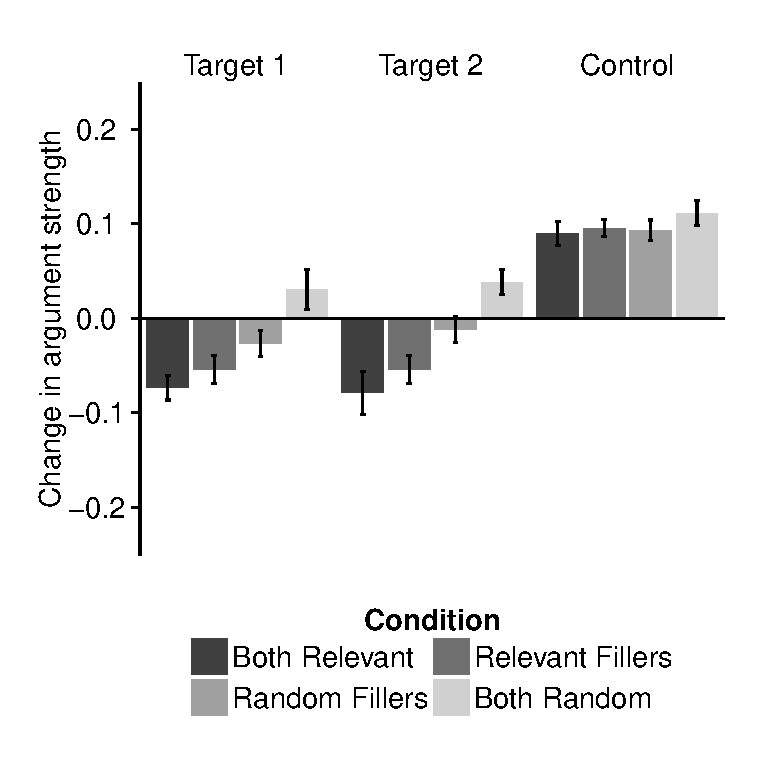
\epsfig{file=results.eps,width=10cm}
% \includegraphics[scale=0.60]{figure1a.eps} &
% %\hspace{-5mm}
% \includegraphics[scale=0.60]{figure1b.eps} \\
% %\hspace{-5mm}
% \multicolumn{1}{c}{\small (a) Model predictions} &
% \multicolumn{1}{c}{\small (b) Human performance}
% \end{tabular}
% \end{center}
% \caption{%
%   (a) Model predictions for the change in argument strength when an additional premise is introduced (i.e., $P(y|x_1,x_2)-P(y|x_1)$).
%   A positive change indicates premise monotonicity, a negative change, non-monotonicity.
%   In the {\bf Control} argument, monotonicity is predicted regardless of sampling assumption. For
%   both {\bf Target} arguments, a reversal is predicted: premise non-monotonicity is
%   expected only under an assumption of strong sampling.\ %
%   (b) Average change in people's argument strength ratings for the \relevant\ and \random\ conditions, calculated by subtracting their original
%   judgment (after seeing the first premise only) from their revised judgment (after seeing the second premise), then
%   linearly scaled to the range -1 to 1. In keeping with the predictions, people exhibit premise non-monotonicity
%   in the \relevant\ condition and only for the {\bf Target} arguments. Bars show standard error.\ %
% }
% \label{fig:results}
% \end{figure}

\begin{figure}[htbp]
\begin{center}
\begin{tabular}{cc}
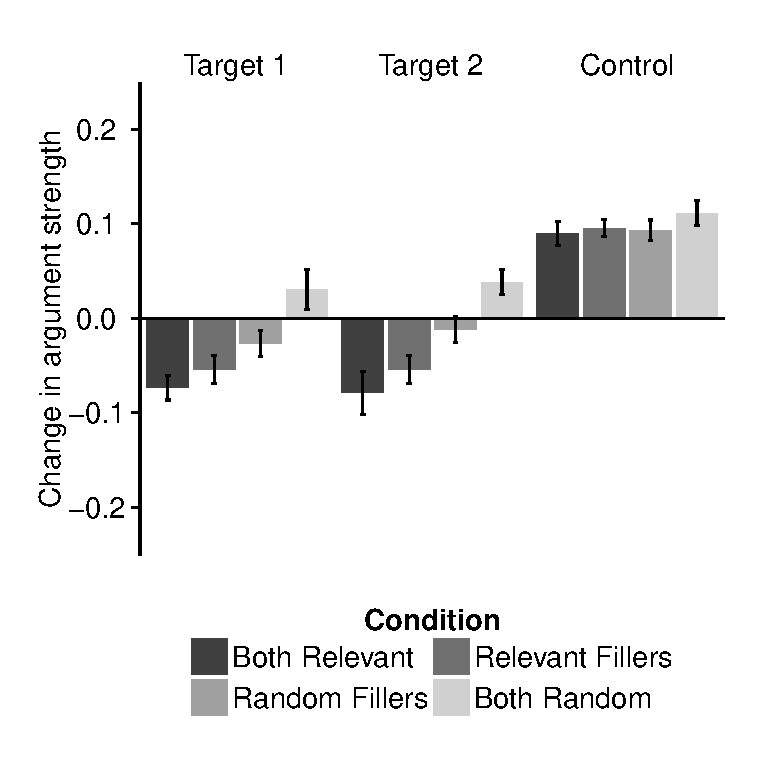
\includegraphics[scale=0.60]{results.eps} &
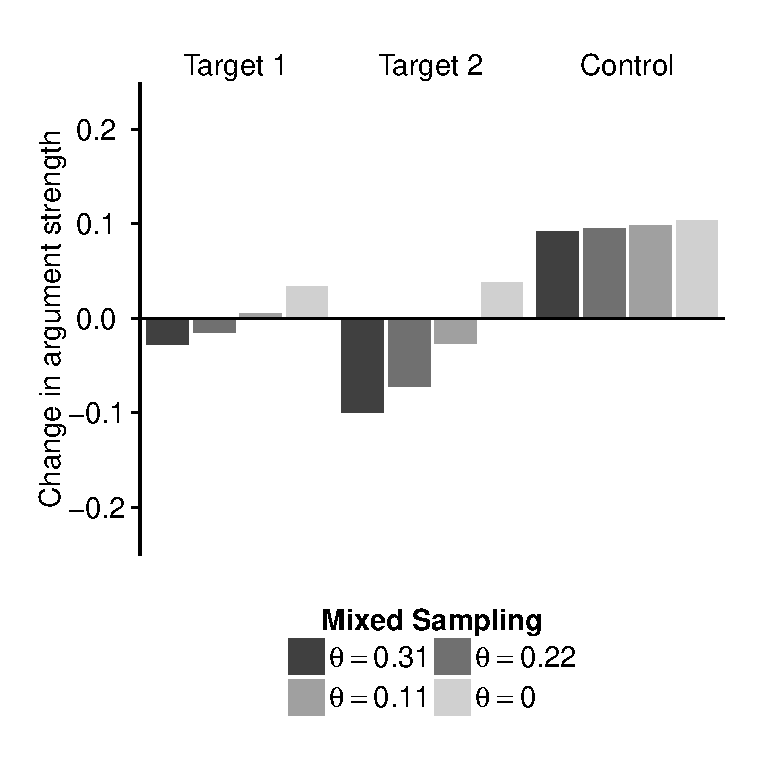
\includegraphics[scale=0.60]{fits.eps} \\
\multicolumn{1}{c}{\small (a) Human performance} &
\multicolumn{1}{c}{\small (b) Model fits}
\end{tabular}
\end{center}
\vspace{-5mm}
\caption{%
   (a) Average change in people's argument strength ratings for all four conditions, calculated by subtracting their original judgment (after seeing the first premise only) from their revised judgment (after seeing the second premise), then linearly scaled to the range -1 to 1.
% TODO: Revisit the next sentence - the graphs shows non-mono in the "random
% fillers" condition, but as pointed out in the text, such a conclusion is not
% well supported by the data.
%
In keeping with the predictions, people exhibit premise non-monotonicity in the \relevant\ and \relevantdata\ conditions and only for the {\bf Target} arguments. The results demonstrate that when a relationship amongst premise categories not shared by the conclusion is highlighted, a strong reason is needed in order for such relevance to be ignored and for non-monotonic reasoning to be inhibited. Bars show one standard error.\ %
%
%  (b) Best fitting value of $\theta$ under a mixed sampling assumption. $\theta=0$ corresponds to assuming that the second item was weakly sampled, $\theta=1$ would correspond to an assumption of pure strong sampling, and intermediate values reflect more graded assumptions. The fitted values confirm that when a cover story establishes a high or low expectation of premise relevance consistent with the premises observed, people exhibit an increased bias towards strong or weak sampling, respectively.\ %
  (b) Best fitting value of $\theta$ under a mixed sampling assumption. $\theta=0$ corresponds to a weak sampling assumption, whereas $\theta=1$ would correspond to an assumption of pure strong sampling. Intermediate values reflect more graded assumptions. The fitted values confirm that when a cover story establishes a high or low expectation of premise relevance consistent with the premises observed, people exhibit an increased bias towards strong or weak sampling, respectively.\ %
}
\label{fig:results}
\end{figure}

\begin{table}[t]
\hspace{-5mm}
\footnotesize
\begin{tabular}{rrrr}
\toprule
 & \multicolumn{3}{c}{Bayes Factor} \\
\cmidrule{2-4}
\multicolumn{1}{c}{Condition} & \multicolumn{1}{c}{Target 1} & \multicolumn{1}{c}{Target 2} & \multicolumn{1}{c}{Control} \\
\midrule
%\relevant\ &  \nonmonowin{150,000}{1} & \nonmonowin{40}{1} & \monowin{$>$ 1,000,000}{1} \\
\relevant\ &  \nonmonowin{$>$ 1,000}{1} & \nonmonowin{40}{1} & \monowin{$>$ 1,000}{1} \\
\relevantdata\ & \nonmonowin{98}{1} & \nonmonowin{91}{1} & \monowin{$>$ 1,000}{1} \\
\randomdata\ & \nonmonodraw{1}{1} & \nonmonolose{1}{5.7} & \monowin{$>$ 1,000}{1} \\
\random\ & \monolose{1}{1.8} & \monowin{13}{1} & \monowin{$>$ 1,000}{1} \\
\bottomrule
\end{tabular}
\vspace{-5mm}
\caption{%
Bayes factors indicating the relative likelihood of a one-sided model of mean change in argument strength against the null model, by condition and trial type. The one-sided test performed in each case (given in parentheses) was chosen on the basis of the mean change in argument strength observed. $\mu<0$, $\mu=0$ and $\mu > 0$ correspond to the hypotheses that the true mean change in argument strength represents non-monotonic, strictly flat and monotonic responding, respectively. Bold type indicates the preferred model in each case. As predicted, a cover story consistent with a strong sampling assumption lead to non-monotonic responding in the {\bf Target} trials, but not the {\bf Control} trial, while a cover story consistent with a weak sampling assumption induced monotonic responding across all conditions and trials. Bayes factors are shown to two significant figures.
}
\label{tbl:monobayesfactors}
\end{table}

% > nonMonoBF(e1, mono1)
%          PP1          CP1          CP2          WP2
% 1.503707e+05 9.810819e+01 9.621409e-01 1.481159e-02
% > nonMonoBF(e2, mono2)
%         PP1         CP1         CP2         WP2
% 39.88324811 91.19043368  0.17581912  0.07237647
% > monoBF(c1, mono3)
%          PP1          CP1          CP2          WP2
% 5.120679e+07 2.380115e+15 2.452901e+11 8.176473e+10

%Figure~\ref{fig:results}(b) shows that, as predicted, people exhibited different response patterns depending on their sampling assumptions. For both {\bf Target} trials, participants in the \random\ condition exhibited premise monotonicity, while those in the \relevant\ condition showed non-monotonicity ({\bf Target 1:} Bayes factor: 441:1 in favour of an effect of sampling condition; {\bf Target 2:} Bayes factor: 971:1).\footnote{Bayes factors reported are for the Bayesian $t$-test and were calculated using the BayesFactor package in R (Morey \& Rouder, 2014, v 0.9.7). Welch's two-sample $t$-tests, confirmed these conclusions, yielding ($t$(217) = -4.15, $p$ $<$ .001) for {\bf Target 1} and ($t$(214) = -4.42, $p$ $<$ .001).} For the {\bf Control} trials, also as expected, different sampling assumptions had no significant effect (Bayes factor 3.9:1 in favour of a null effect).\footnote{A Welch's two-sample $t$-test failed to reject the null hypothesis for the Control trial ($t$(264) = -1.15, $p$ $>$ .05).}  In fact, the effect of sampling assumption on premise monotonicity in our experiment was strong enough to cause a genuine reversal in whether people were prepared to endorse the conclusion in one case. For the second target trial 78\% of participants in the \random\ condition endorsed the conclusion that lions produce the hormone TH-L2, compared to 37\% in the \relevant\ condition. With respect to the first target trial the effect was less pronounced due to low overall endorsement of the conclusion; 24\% endorsement in the \random\ condition compared to 11\% in the \relevant\ condition.

\cref{fig:results}(a) shows, as predicted, that people exhibited different response patterns depending on their sampling assumptions. For both {\bf Target} trials, participants in the \random\ condition exhibited premise monotonicity, while those in the \relevant\ condition showed non-monotonicity.
%(\relevant: {\bf Target 1:} Bayes factor: 150,000:1 in favour of a non-monotonic change in argument strength against no change; {\bf Target 2:} Bayes factor: 40:1; \random: {\bf Target 1:} Bayes factor: 1.8:1 in favour of no change in argument strength against a monotonic change; {\bf Target 2:} Bayes factor: 13:1 in favour of a monotonic change).
To quantify the amount of evidence for these assertions, for every condition we ran Bayesian analysis comparing three hypotheses: that responding was monotonic (positive change: $\mu>0$), non-monotonic (negative change: $\mu<0$) or that the additional premise had no influence (null effect: $\mu=0$). Analyses were conducted using the BayesFactor package in R \cite{MR14}, applying the method outlined by \citeA{MW14} to test one-sided hypotheses. The results of these analyses are summarized in \cref{tbl:monobayesfactors}, which reports the Bayes factor between the two best hypotheses in each case. As the table makes clear, there is strong evidence for monotonic reasoning on the control trials regardless of condition, but there is evidence for a shift from monotonic to non-monotonic reasoning in the target conditions.



For the two conditions employing a neutral cover story, our intuition was that a mixed sampling assumption should be induced. Consequently, we expected mean response change in the \relevantdata\ and \randomdata\ conditions to be within the bounds of that for the \relevant\ and \random\ conditions. To investigate this intuition, we determined the mix of strong and weak sampling assumptions (captured by $\theta$, as per \cref{eqn:mixedsampling}) that best fit the mean response change observed for each condition. The fitting process involved finding a value for $\theta$ (in the range 0 to 1) that minimised the squared difference between predicted response change and mean observed response change summed across {\bf Control} and {\bf Target} trials.

As \cref{fig:results}(b) shows, the change in relative mixture across conditions follows the expected pattern. The correlation between fitted model and data is 0.94, indicating a good fit overall.
%
Further analysis showed that order restricted models suggesting either an effect of cover story only or both cover story and filler items were both well supported by the data, with the latter having strongest support overall (Bayes factors are shown in \cref{tbl:modelbayesfactors}).
%({\bf Target 1:} Bayes factor: 2900:1 in favour of an effect of cover story and filler items against the null ; {\bf Target 2:} Bayes factor: 29600:1).
Bayes factors were calculated using a custom JAGS model, employing the product space method of model comparison (\citeNP{LKLT11}; see Appendix B for details).

\begin{table}[t]
\hspace{-5mm}
\begin{tabular}{lcrrr}
\toprule
 & & \multicolumn{3}{c}{Bayes Factor ( : {\textsc{no effect}})} \\
\cmidrule{3-5}
Model & Order restrictions & Target 1 & Target 2 & Control \\
\midrule
\textsc{no effect} & $ \mu_1 = \mu_2 = \mu_3 = \mu_4$ & - & - & - \\
\textsc{fillers only} & $ \mu_1 = \mu_2 < \mu_3 = \mu_4$ & 740:1 & 12,000:1 & $< 1:1$ \\
\textsc{story only} & $ \mu_1 < \mu_2 = \mu_3 < \mu_4$ & 4,100:1 & 17,000:1 & $< 1:1$ \\
\textsc{both} & $ \mu_1 < \mu_2 < \mu_3 < \mu_4$ & 2,900:1 & 30,000:1 & $< 1:1$ \\
\textsc{random effect} & $ \mu_1 \neq \mu_2 \neq \mu_3 \neq \mu_4$ & 520:1 & 4,600:1 & $< 1:1$ \\
\bottomrule
\end{tabular}
\caption{%
Bayes factors representing the relative likelihood of the observed changes in argument strength under each model compared with the \textsc{no effect} model. A higher Bayes factor indicates greater evidence in favour of a particular model. Each model is described in terms of the order restrictions amongst the values $\mu_1$, $\mu_2$, $\mu_3$ and $\mu_4$, which represent the true means of the $\relevant$, $\relevantdata$, $\randomdata$, and $\random$ conditions, respectively. Bayes factors are shown to two significant figures.
}
\label{tbl:modelbayesfactors}
\end{table}

% > r$f1$BF; r$s1$BF; r$b1$BF; r$u1$BF
% [1] 738.9897
% [1] 4115.886
% [1] 2878.796
% [1] 519.6272
% > r2f2$BF; r2s2$BF ; r2b2$BF ; r2u2$BF
% [1] 12458.05
% [1] 16517.9
% [1] 29595.54
% [1] 4568.756
% > r3$f3$BF ; r3$s3$BF; r3$b3$BF; r3$u3$BF
% [1] 0.4815399
% [1] 0.3469041
% [1] 0.06414061
% [1] 0.05275805

Overall, the effect of sampling assumption on premise monotonicity in our experiment was strong enough to cause a genuine reversal in whether people were prepared to endorse the conclusion in one case. For the second target trial 78\% of participants in the \random\ condition endorsed the conclusion that lions produce the hormone TH-L2, compared to 37\% in the \relevant\ condition. With respect to the first target trial the effect was less pronounced due to low overall endorsement of the conclusion; 24\% endorsement in the \random\ condition compared to 11\% in the \relevant\ condition.

\section{Discussion}

% My overall goal for this section was to answer:
%
% What did we find?
% How is that novel?
% What do our results build on/conflict with?
% What models/theories can explain our results?
% What does it all mean?
% Where to from here?

% Basic recapitulation of what we found
%
Arguments, when presented in everyday life, are intended to bring about a change in the audience. Whether to engage, to teach or persuade, premises are typically selected with a relevant goal in mind.
% Revision
This paper investigates why premise relevance should matter when people evaluate arguments.
%
We demonstrate that people's reasoning in a \cbi\ task is dependent on their assumptions about how the premises were sampled. If they think the premises were provided by a helpful confederate choosing positive examples from the categories in question, they show the premise non-monotonicity effect found previously \cite{MCSH03}. However, if they believe that the premises were generated randomly, this effect reverses. These results can be explained by a Bayesian theory of \cbi\ that naturally incorporates different assumptions about premise sampling.

% Teasing out two different conclusions
%
Our results support two qualitatively different conclusions. First, our work shows that the perceived strength of an inductive argument is influenced not just by the direct generalizability of premises to conclusion,
% Revision
but also by expectations of premise relevance. By inducing a weak sampling assumption we showed that sensitivity to premise relationships can be violated.
%
Second, this influence is pronounced enough to lead to a reversal of an effect (premise non-monotonicity) that normally obtains for certain kinds of argument structures.  Reasoners who hold different sampling assumptions may endorse opposite conclusions as a result.

%Our findings build upon and extend the experimental work of \citeA{Fer06}, who also found that varying sampling assumptions affected inductive argument strength. However, that research did not find the standard reversal of premise

% Relationship with what Fernbach found plus importance of cover story
%
A previous attempt by \citeA{Fer06} to demonstrate premise non-monotonicity by inducing a weak sampling assumption was not entirely successful. Although \citeA{Fer06} found a difference in argument strength depending on sampling assumptions, participants in that study did not show a qualitative shift from monotonic to non-monotonic reasoning. Instead, the additional premises raised argument strength in all cases.  It is possible that the relevance of the additional premises was not clear enough in that manipulation, which did not vary filler items. In our experiment we used filler items to substantiate the cover story in the \relevant\ and \random\ conditions. For example, our \random\ condition contained negative examples as filler items, without which a weak sampling assumption is difficult to sustain.  Previous work involving category learning has also found that people rely on data, not just cover stories, to determine which sampling assumptions are appropriate. For instance, \citeA{NDL12} found that the data people were shown affected their generalizations, but that sampling assumptions implicit in the cover story did not. A replication of that study which made the sampling assumptions in the cover story more explicit did find a reliable effect of cover story \cite{VHPN13}. Our results showed a reliable effect of both cover story and filler items, with participants in the \relevantdata\ and \randomdata\ conditions exhibiting a similar, albeit attenuated, pattern of responding to those in the \relevant\ and \random\ conditions, respectively. This lends further support to the intuitive notion that in many cases people's sampling assumptions reflect some weighted mixture of strong and weak sampling. And while the questions remains open as to whether and how sampling assumptions are updated as new data arrives, it is clear that people do pay attention to the nature of the data when determining how that data was generated.

%Our analyses demonstrates that when a relationship amongst premise categories
%not shared by the conclusion is highlighted, a strong reason is needed in
%order for such relevance to be ignored and for non-monotonic reasoning to be  inhibited.

% Dealing with where similarity fits in
%
Prominent models of inductive argument strength, such as the similarity-coverage model of \citeA{Osh90}, and the featural similarity model of \citeA{Slo93} suggest that argument strength is based on the similarity between premise and conclusion, as first observed by \citeA{Rip75}. However, these models offer no explicit mechanism to capture sampling assumptions. Each model ``hard-wires'' a particular assumption instead. In contrast, as we have shown, a Bayesian model along the lines we have illustrated can accommodate the roles of both premise-conclusion similarity and sampling assumptions.

% Revision: dealing with relevance theory
%
How might the relevance framework for inductive reasoning \cite{WS04} accommodate our finding that premise sampling assumptions affect argument strength? Relevance theory claims that an input is worth picking out from the mass of competing stimuli when it is {\em more} relevant, and that an input is more relevant if it produces a larger cognitive effect or requires less effort to process. The addition of a premise that highlights a shared property should raise the relevance of that property when determining the appropriate basis for induction, by decreasing the effort required to call the property to mind. But that should be so in each of our experimental conditions, because identical premises were used in the trials of interest. So that leaves us to posit a difference in cognitive effect to explain a difference in relevance between conditions.

This is where the Bayesian theory of \cbi\ comes in. The theory describes how beliefs are revised in response to evidence in terms of the redistribution of probability mass. Such redistribution, we argue, is an excellent candidate measure for cognitive effect. Under this view, the mathematics of Bayes' rule predicts that a strong sampling assumption will always lead to a greater cognitive effect than would a weak sampling assumption because it leads to belief revision due to differences in the likelihood of observing certain data, and not simply due to falsification alone.\footnote{An important implication of this assumption is that equating cognitive effect directly with change in argument strength is potentially flawed, since the two forms of belief revision can have opposing effects.} Relevance theory holds that comparing stimuli on the basis of relevance is a crucial part of human reasoning. The Bayesian theory of \cbi\ provides a computational basis for making such comparisons in a way that takes two critical factors -- premise sampling assumptions and category similarity -- into account. As such, the theory represents an important component that can be integrated into the relevance framework. Likewise, relevance theory complements Bayesian theory insofar as it can make qualitative predictions regarding processing effort. Any algorithmic account of \cbi\ should take these predictions into account, as well as relevant empirical findings \cite<e.g.>{CV10,FCC10,FH11}.

% Half hearted attempt at a link to relevance theory
%
In general, we found that people in our experiment quite naturally assumed that premises were selected sensibly or drawn from the category -- the difficulty came in trying to persuade them that they were truly random, as in the \random\ condition. This observation, in combination with the fact that the premise non-monotonicity found in the \relevant\ condition corresponds to the standard effect \cite{MCSH03}, suggests that people have an automatic bias to believe that premises are selected sensibly: if not by a helpful teacher, at least in a way consistent with strong sampling (i.e., selected from the category).
% Revision
%
A biased presumption of relevance is an outcome in keeping with a central claim of relevance theory that people act to maximise relevance when selecting inputs to process \cite{WS04}. This is sensible in the context of \cbi\ given that this is how arguments are constructed and used in the real world, but it does mean that we cannot, as researchers, assume that people reason as if we are generating examples randomly (even when we are).

% Strong versus pedagogical
%
It should be noted that our model incorporates strong sampling, which in the context of \cbi\ implies that a category exhibiting the property in question is as likely as any other to be chosen.
% Revision
Seeking to persuade or dissuade another is typically a matter of picking a relevant example of a concept, not a random one. Yet, when a property defines a small or coherent category such as ``species of bear'' or ``black and white striped animals'' then there is likely to be little variation in relevance across the category members, and a strong sampling assumption may be appropriate. A pedagogical assumption, in contrast, which gives greater weight to examples that better characterise a property, may be more appropriate for larger, less coherent categories, where there is greater variation in relevance across category members.\footnote{Pedagogical sampling \cite{SGG14} may be viewed as a partial instantiation of the {\em communicative principle of relevance} \cite{WS04}, insofar as it can make predictions about belief revision in an explicitly communicative context.}
%
\citeA{SGG14} found evidence to suggest that pedagogical sampling compared to strong sampling lead to tighter generalizations on the part of the learner, albeit with simple perceptual stimuli. It is plausible that our \relevant\ cover story acted to tighten generalizations over and above the predictions of strong sampling. Such a tightening may have acted to increase levels of premise non-monotonicity in the \relevant\ condition. Further work is needed to determine whether premise non-monotonicity can be observed with a cover story suggestive of a strong sampling assumption alone, in line with our model simulations. Regardless, the likelihood function in the Bayesian model may be adapted to capture either strong or pedagogical sampling \cite{SGG14}.

% Wrap-up: with an emphasis on strong sampling
%
There is substantial evidence to suggest that when attempting to learn, generalize and draw conclusions from data, people are sensitive to the process by which data is generated. This sensitivity to sampling has been previously shown in simple generalization problems \cite{TG01,NDL12}, in early word learning \cite{XT07}, and even in infants \cite{GHT10}. Other work has demonstrated that people are sensitive to more complicated sampling schemes \cite{SGG14}.
% Revision
Our work extends this sensitivity to \cbi\ tasks, adding an important clarification to relevance theoretic accounts of a phenomena attributed to relationships amongst premise items. In a world of exclusively weak sampling assumptions, where evidence supports falsification only, the inferential leap receives no boost from premise relevance: the relevant becomes irrelevant.

\section{Appendix A}
\label{sec:derivingpriors}

In order to generate model predictions (using \crefrange{eqn:bayes}{eqn:strongsampling} described in the main paper) it is necessary to specify an hypothesis space $\bigh$ and a prior distribution, $P(\bigh)$. To do so, we restrict the category labels under consideration to the fourteen experimental stimuli used in both experimental conditions. This is not to say that the experimental participants were aware in advance of the nature and extent of the stimuli used, nor restricted their considerations in this manner. We made this restriction to render analysis tractable, with the view that the predictions remain valid in a qualitative sense, despite this truncation. The fact that our experimental results match our predictions in qualitative terms lends support to this view. Given the fourteen category labels, our hypothesis space $\bigh$ consists of $2^{14}$ hypotheses, each corresponding to the proposition that a unique cluster of categories share a given property.

Having established our hypothesis space $\bigh$, we need to separately derive a plausible prior distribution, $P(h)$, defined over all $h \in \bigh$. We seek a prior that is independent of any particular property or this specific task, to avoid fitting our predictions too tightly to the properties used in our experimental trials. That is, $P(h)$ represents the probability that a blank (unseen) property is shared by those items that belong to a particular category $h$. In keeping with prominent models of category-based induction \cite{Osh90, Slo93}, we assume that generalizing a property from one item to another involves an assessment of their similarity. Intuitively, since hypotheses in our model correspond to clusters of items, we seek to establish a weighting for each cluster that reflects its coherence. Prior probabilities will be derived from these clusters, with higher prior probabilities assigned to more coherent clusters.

To establish clusters and associated weights we apply the {\em additive clustering} (ADCLUS) model \cite{SA79,Lee02,NG08} to similarly data gathered from a separate experiment, described in more detail below. On the basis of observed similarity data, ADCLUS identifies structure in the domain free from the undesirable restriction that such structure take a strictly hierarchical form.
The model defines the similarity of any two objects as the sum of the weights across all clusters containing both objects. It attempts to find a set of clusters and weights maximising the fit between empirical similarity data and the theoretically reconstructed measures. Finding an optimal fit is an under-constrained and computationally expensive exercise, hence the model implementation seeks to find a good and parsimonious fit. Starting with an initial configuration of clusters and weights, a gradient descent algorithm is employed to find a suitable local optimum. On each iteration of the gradient descent process, clusters with non-appreciable weights may be discarded.

In order to provide empirical interstimulus similarities as input to the ADCLUS model, a separate experiment was conducted to gather similarity ratings via a triad task for the fourteen animal stimuli common to all conditions of our experiment. 63 adults were recruited via Amazon Mechanical Turk, and were each paid \$0.60 (USD) for the 5--10 minutes participation. 5 were excluded due to browser incompatibility, and the remaining 58 were aged 19 to 75 years (median age 31, 41\% female). 50 participants were in the United States, with 8 located elsewhere. For each triad presented, people were asked to pick which animal was {\em least} similar to the others. Each person rated 60 randomly selected triads. Since there were a total of 364 possible triads, this meant that each triad was rated by 9--10 participants on average. The pairwise interstimulus similarity for two stimuli $a$ and $b$ was calculated as the proportion of all triad ratings for $a$, $b$, and some other stimulus $c$, where $c$ was rated as being the least similar.

The final stage in our model implementation involves the assignment of prior probabilities based on the clusters and weights identified by ADCLUS. Let $\bigh_C$ denote those hypotheses (clusters) identified by the ADCLUS process, and $w_h$ denote the weight associated with hypothesis $h \in \bigh_C$. We form an initial estimate of the prior distribution directly from these outputs:

\begin{equation}
P_w(h) \propto \left\{
  \begin{array}{l l}
    w_h & \quad \textrm{if $h \in \bigh_C$} \\
    0 & \quad \textrm{otherwise}
  \end{array} \right.
\end{equation}
This initial estimate is not quite right, however. The ADCLUS model does not deal meaningfully with clusters corresponding to a single category. Yet intuitively, in the context of our experiment, properties that pertain to a single category (\category{Tiger}, for example) are quite plausible. Therefore we need to combine the prior derived from the cluster weights with one that assigns non-zero probability to the singleton hypotheses (the set of which we denote $\bigh_S$). For the latter, we use a size-based prior:
\begin{equation}
\label{eqn:sizeprior}
P_s(h) \propto \left\{
  \begin{array}{l l}
    \frac{1}{|h|} & \quad \textrm{if $h \in \bigh_C \cup \bigh_S$} \\
    0 & \quad \textrm{otherwise}
  \end{array} \right.
\end{equation}
Lastly, we combine these two prior distributions to form the prior used to generate our model predictions in such a way that the probabilities for singleton hypotheses calculated in \cref{eqn:sizeprior} are preserved:
\begin{equation}
\label{eqn:finalprior}
P(h) = \left\{
  \begin{array}{l l}
    P_s(h) & \quad \textrm{if $h \in \bigh_S$} \\
    P_w(h) \sum_{h^\prime \in \bigh_C} P_s(h^\prime) & \quad \textrm{if $h \in \bigh_C$} \\
    0 & \quad \textrm{otherwise}
  \end{array} \right.
\end{equation}
As the reader will note, our method for defining the hypothesis space and for deriving prior probabilities affords a certain latitude. Using the ADCLUS model, the precise clusters and associated weights identified depend on the values chosen to seed the optimization process. Whilst we retain the seeding heuristic of \citeA{SA79}, we also experimented with other heuristics. We found that although such alternatives lead to different numerical predictions, the important qualitative effect was robust: greater levels of premise non-monotonicty were predicted under a strong sampling assumption than under a weak sampling assumption for the {\bf Target} (but not the {\bf Control}) arguments. Similarly, alternative methods may be employed for assigning probabilities to singleton hypothesis, but once again, the qualitative predictions appear robust in the face of such changes.

% ADCLUS defines the notion of an {\em elevated subset} representing a
% cluster $A$ that satisfies:
% \begin{equation}
% \label{eqn:elevatedset}
% B \supset A \Rightarrow \min_{i,j \in B}s(i,j) < \min_{i,j \in A}s(i,j)
% \end{equation}
% where $s(i,j)$ represents the interstimulus similarity of $i$ and $j$. Intuitively, if minimum interstimulus similarity is a measure of cluster coherence, then an elevated subset corresponds to a cluster that can only be made less coherent by the addition of further members. This notion is similar to that of {\em compactness} used in {\em complete link clustering}, a commonly employed form of hierarchical clustering.

\section{Appendix B}

As discussed in the main text, differences in mean change in argument strength across conditions indicated that our experimental manipulation had some effect.
To investigate the factors driving the effect we compared a number of plausible models to determine which might best account for our experimental results. The models considered were based on the change in argument strength predicted by our Bayesian model of \cbi, derived from empirical similarity ratings. Under a strong sampling assumption, our model predicts non-monotonic responding for both {\bf Target} trials; under a weak sampling assumption, monotonic responding is predicted.

Furthermore, the fitted values of $\theta$ derived from the mixed sampling model suggest an ordering in terms of mean  response change across conditions. Thus, consistent with the suggested orderings, three plausible models concerning the nature of the effect were compared, namely: that the effect was driven by the filler items only (\textsc{fillers only}), that it was driven by the cover story only (\textsc{story only}), or that it was driven by both of these factors (\textsc{both}). The order restrictions for each model are shown in \cref{tbl:betavalues}. A fourth unrestricted model was also considered, namely that results were driven by a random effect (\textsc{random effect}).

For each of the four models, we calculated the Bayes factor representing the relative likelihood of the observed changes in argument strength under the model against the ``no effect'' model (\textsc{no effect}). To do so, we employed a Markov chain Monte Carlo (MCMC) procedure known as the {\em product space method} \cite{LKLT11}. The technique supports the comparison of two models ($M_o$ and $M_1$, for example) by building a hierarchical ``supermodel'' combining the models via a random variable ($M$, say) that acts as a model index. The Bayes factor for the relative likelihood of $M_1$ against $M_0$ becomes the posterior odds ratio ($M_1$ : $M_0$) for the two models, divided by the prior odds ratio. Theoretically, the prior model probabilities may be chosen with freedom, although technical considerations require careful selection if reliable MCMC estimates are to be obtained. Finally, the prior probabilities for each model may be estimated as follows:
\begin{equation}
\label{eqn:modelposterior}
\hat{P}(M_k \given \textrm{Data}) = \frac{\textrm{Number of posterior samples where $M = k$}}{\textrm{Total number of posterior samples}},
\end{equation}
from which the Bayes factor easily follows.

\begin{figure}[t]
\begin{minipage}{0.5\textwidth}
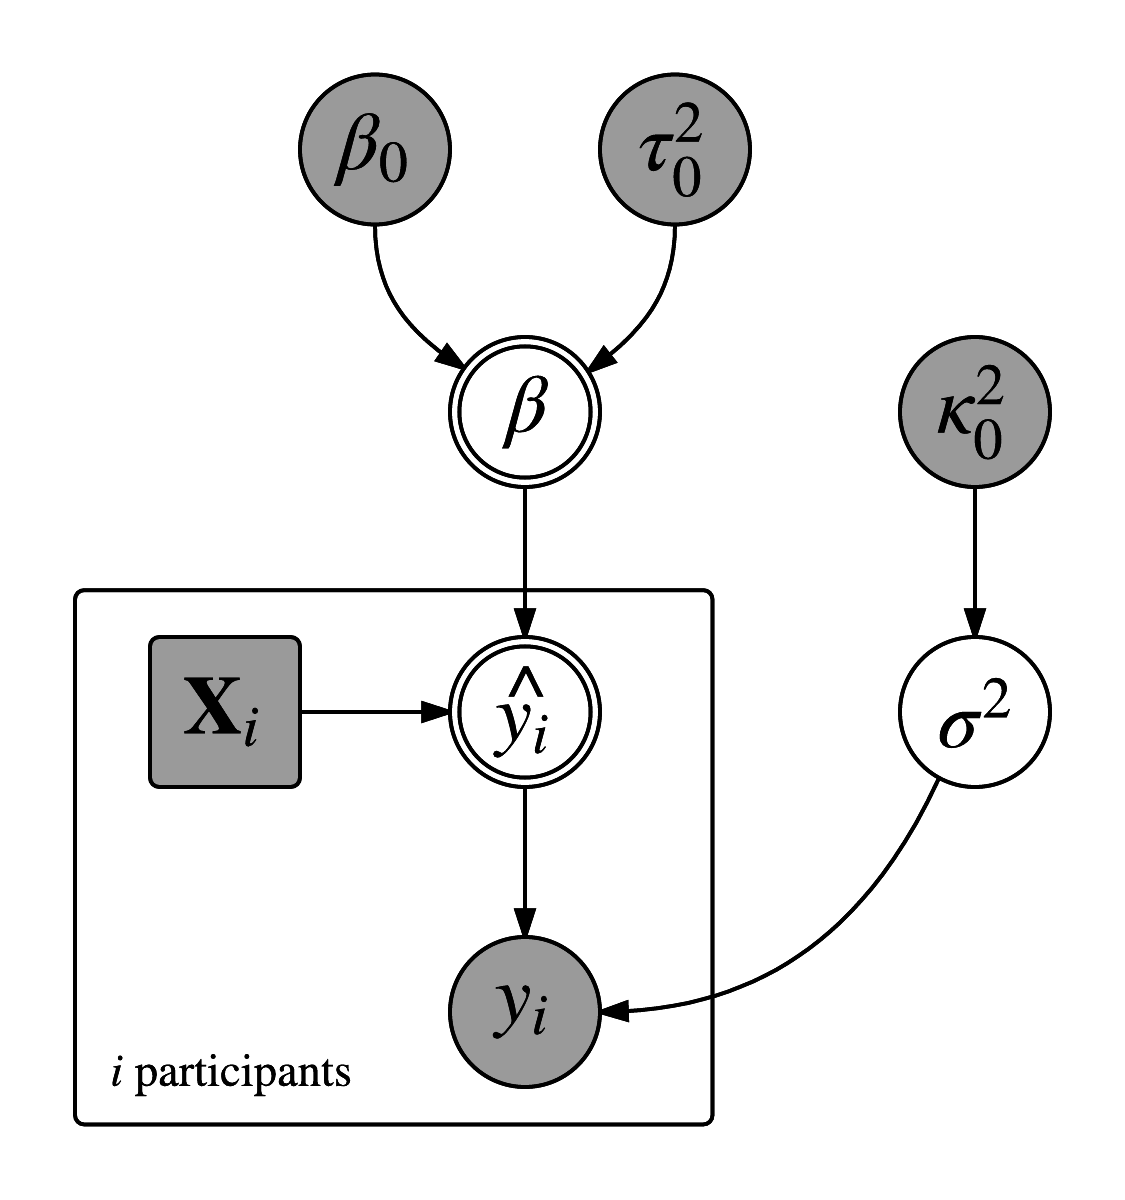
\includegraphics[scale=0.80]{graphicalmodel.png}
\end{minipage}
\begin{minipage}{0.5\textwidth}
\begin{eqnarray*}
\phantom{a} & \\[-10mm]
y_i &\sim& \textrm{Normal}\big(\hat{y_i}, \sigma^2\big) \\[\jot]
\hat{y_i} &=& \beta_1 + \beta_2 X_{1i} + \beta_3 X_{2i} + \beta_4 X_{3i}  \\[\jot]
%\frac{1}{\sigma^2} &\sim& \Gamma\Big(\frac12 , \frac{\kappa_0^2}{2}\Big) \\[3mm]
\sigma^2 &\sim& \textrm{Scaled Inverse}\ \chi^2\big(1, \kappa_0^2\big) \\[\jot]
\beta_1 &\sim& \textrm{Normal}\big(\beta_0, \tau_0^2\big) \\[\jot]
\beta_2 &=& \delta_1 \\[\jot]
\beta_3 &=& \delta_1 + \delta_2 \\[\jot]
\beta_4 &=& \delta_1 + \delta_2 + \delta_3
\end{eqnarray*}
\end{minipage}
\caption{%
A graphical model supporting comparison of condition means. For each of the five models considered, $\beta_1$ represents the condition mean of the reference condition \relevant. $\beta_2$, $\beta_3$, and $\beta_4$, represent the difference between the mean of the reference condition and the mean of the \relevantdata, \randomdata, and \random\ conditions, respectively. The models differ only in the definition of $\delta_1$, $\delta_2$, and $\delta_3$.
}
\label{fig:graphicalmodel}
%\vspace{-5mm}
\end{figure}

\Cref{fig:graphicalmodel} shows the graphical model capturing the common elements for each of the models tested. The vector quantity $\bm{X_i} = (X_{1i}, X_{2i}, X_{3i})$ represents a dummy coding of condition for each participant. The vector quantity $\bm{\beta} = (\beta_1, \beta_2, \beta_3, \beta_4)$ captures the relationship between the means $\mu_1$, $\mu_2$, $\mu_3$, and $\mu_4$ of the \relevant, \relevantdata, \randomdata, and \random\ conditions, respectively; that is, $\beta_1 = \mu_1$, $\beta_2 = \mu_2 - \mu_1$, $\beta_3 = \mu_3 - \mu_1$, and $\beta_4 = \mu_4 - \mu_1$. The $\delta_i$ parameters represent the difference between adjacent condition means, and are each sampled from a normal distribution with mean 0 and variance $\tau_0^2$. The range restrictions on the values sampled differ across the five models, as shown in \cref{tbl:betavalues}. The mean of the reference condition has a normal prior distribution with mean $\beta_0$, and variance $\tau_0^2$. The prior for the error variance ($\sigma^2$) is a scaled inverse $\chi^2$ distribution, with 1 degree of freedom and scaling parameter $\kappa_0^2$. To ensure that these prior distributions do not favour any one particular model, and that the posterior is effectively independent of the prior, the values for $\beta_0$, $\tau_0^2$, and $\kappa_0^2$ were derived from the data using the procedure outlined in \citeA[p. 482]{KLHH05}.

\begin{table}[t]
\hspace{-5mm}
\small
\begin{tabular}{lcccc}
\toprule
 & & \multicolumn{3}{c}{Parameter range} \\
\cmidrule{3-5}
Model & Order restrictions & $\delta_1$ & $\delta_2$ & $\delta_3$ \\
\midrule
\textsc{no effect} & $ \mu_1 = \mu_2 = \mu_3 = \mu_4$ & 0 & 0 & 0 \\
\textsc{fillers only} & $ \mu_1 = \mu_2 < \mu_3 = \mu_4$ & 0 & $(0, \infty)$ & 0 \\
\textsc{story only} & $ \mu_1 < \mu_2 = \mu_3 < \mu_4$ & $(0, \infty)$  & 0 &
$(0, \infty)$ \\
\textsc{both} & $ \mu_1 < \mu_2 < \mu_3 < \mu_4$ &
$(0, \infty)$ &
$(0, \infty)$ &
$(0, \infty)$ \\
\textsc{random effect} & $ \mu_1 \neq \mu_2 \neq \mu_3 \neq \mu_4$ &
$(-\infty, \infty)$ &
$(-\infty, \infty)$ &
$(-\infty, \infty)$ \\
\bottomrule
\end{tabular}
\caption{%
The range restriction imposed on the Normal$\big(0, \tau_0^2\big)$ distribution from which the $\delta_i$ parameters are sampled for each model. A value of $0$ indicates that the respective parameter is always $0$.
}
\label{tbl:betavalues}
\end{table}

% end of content
% ------------------------------------------------------------------------


% finish
\bibliography{paper}
\bibliographystyle{apacite}
\end{document}





%  LocalWords:  xtable

% previously used text fragments:

% From Intro

% CUT: Under a naive model of human cognition, whereby reasoning proceeds
% deductively, learning is a process of encountering, encoding and storing the
% facts and rules that may be used in subsequent logical reasoning. Under this
% model, all knowledge is certain; propositions either ``true'' or
% ``false''. When faced with new information, beliefs are either confirmed or
% confounded, there is no moderation. The context in which information is
% acquired is not relevant. Everyday reasoning, in contrast, is typically {\em
% inductive}, drawing as it does upon incomplete information in order to reach
% probable yet uncertain conclusions. Where knowledge is not certain but
% probabilistic, the role of learning seems better described as the acquisition
% of evidence used to fuel predictions and to assess the plausibility of such
% predictions (whether one’s own or those of others). Which raises an
% interesting question - what processes govern the assessment of plausibility?
% The study of inductive inference and inductive generalization are attempts at
% tackling this question, central to the field of cognitive science. Much
% research has focused on the nature of evidence and its relationship to the
% target of generalization, as well as pre-existing biases that might make some
% properties more readily inferred than others. Though critically important,
% assumptions made by the reasoner about the evidentiary value of data gathered
% in a particular context, have received less attention. The research described
% in this paper represents a novel demonstration that changes in these
% assumptions may directly affect inferences made in a \cbi\
% task.

% Even when considering blank (unknown) categories and blank features, the
% predictions of \monop\ may seem plausible by considering sample size
% only. If one reasons along the lines ``I knew of one category of object in the
% world with the given feature, I now know of another'', it is not unreasonable
% to increase one’s belief that there may yet be a third category
% \footnote{similar logic may be followed in the case of a negative premise}.

% Intuitively, everyday inductive reasoning seems sensitive to assumptions made
% by the reasoner regarding the evidentiary value of data, so-called sampling
% assumptions. Previous work has demonstrated such sensitivity when performing
% simple categorsation tasks and generalizations based on perceptual stimuli. We
% investigate whether such sensitivity is shown using a \cbi\
% task, which is thought to involve a more complex process of inference than a
% single generalization judgement. We begin by examining the phenomenon of
% \nonmono\ responding and demonstrate how a functional Bayesian account of
% \cbi\ predicts greater scope for \nonmono\ responding under
% a strong sampling assumption than under a weak one. We then present an
% experiment designed to test this conjecture by attempting to directly
% manipulate sampling assumptions between experimental conditions. Our main
% finding is that the evidentiary value of data in the form of additional
% premises is context-dependent in a \cbi\ task. We conclude
% with a discussion of the psychological meaning of these results, and outline
% areas for further investigation.

% Cut from intro to category-based induction and monotonicty

% CUT: \citeA{Osh90} for example, noted that an argument projecting a property
% from \category{Fly} to \category{Bee} was rated stronger than one projecting
% from \category{Fly} and \category{Orangutan} to \category{Bee}. Various
% explanations of premise non-monotonicity have been offered. \citeA{MCSH03}
% posit that adding premise categories might weaken an argument if the added
% categories reinforce a property shared by all premise categories but not by
% the conclusion category. \citeA{Osh90}

% CatBasedIndReview2010 mentions \nonmono\ via property reinforcement - the
% addition of premises that highlight a distinctive relationship reduces
% generalization to other categories.  Osherson: non-mono specific
% (Fly/Bee). Non-mono general. Explanation relates to similarity component and
% coverage component structured stats model paper raises conjecture that
% sample size leads to non mono (and cites sanjana and tennenbaum
% 2003). Wouter’s paper on negative evidence also raises same speculation.

% Cut from Bayesian model section

% The motivation behind this research is to test the hypothesis that sampling
% assumptions matter in the context of a \cbi\ task, a
% semantically rich and relatively naturalistic task setting. In particular
% whether differential levels of non-monotonic responding can be induced through
% the manipulation of sampling assumptions.  Furthermore, we seek to identify a
% model of the computational problem \cite{Mar82} facing the reasoner in this
% context, capable of generating plausible predictions in line with the
% hypothesis.

% CUT: We seek to demonstrate that a Bayesian model, in contrast, can
% accomodate the roles of both premise-conclusion similarity and sampling
% assumptions.

% CUT: In contrast, Bayesian theory, which provides a principled way in which
% the strength of belief in a conclusion can be linked to the evidence observed,
% allows sampling assumptions to be explicitly captured.

% CUT: We model evidence as being definitive, letting $h \Rightarrow x$ denote
% the case where the hypothesis $h$ and evidence $x$ are {\em
% consistent}. Specifically, $h \Rightarrow x$ when $x \equiv +c : c \in h$ or
% $x \equiv -c : c \notin h$.

% CUT: The first term, $P(\data \given h)$, known as the likelihood function,
% provides the means for capturing sampling assumptions. The intuition behind
% this follows.  If we hold a hypothesis true, and consider how data is being
% sampled, we will see that there is a range of observations that would be
% consistent with (that is, {\em predicted by}) the hypothesis. These
% observations may be positive, as in ``\category{X} has the property'', or
% negative, as in ``\category{X} does {\em not} have the property''). The
% likelihood function then, represents the chances that one particular
% observation was made out all of the observations that could have been made if
% the hypothesis were true. Under weak sampling, where the sampling of one item
% of data is no more likely than another, the likelihood function represents a
% constant value for all hypotheses consistent with the data. This implies that
% after observing an item of data, all hypotheses consistent with the data
% retain the same relative plausibility as before. Under strong sampling, if an
% hypothesis consistent with the data observed is consistent with $|h|$ items of
% data in total, then the likelihood function is $\frac{1}{|h|}$. In this case,
% hypotheses consistent with the data do not retain the same relative
% plausibility after the observation is made; instead, smaller hypotheses (those
% predicting fewer consistent observations) become relatively more plausible.

% CUT: Firstly let us make two assumptions:
% \begin{enumerate}
% \item all hypotheses are conceived a priori, and
% \item with respect to a given observation, all hypotheses may be judged either
%   consistent or inconsistent.
% \end{enumerate}
% Whilst we do not claim these as universal truths, we maintain that In the
% context of a \cbi\ task, these assumption hold to a degree
% sufficient to make the subsequent analysis of interest. Proceeding from these
% assumptions, we see that one of two things should happen with regard to our
% belief in a particular hypothesis upon the observation of data: if the
% hypothesis is inconsistent with the data then we reject the hypothesis, thus
% $P(h \given \data) = 0$; if the hypothesis is consistent with the data then we
% update our belief accordingly.
%
% Under a weak sampling assumption, there is no change in the relative
% plausibility of any hypothesis remaining consistent with the data, therefore
% belief in that hypothesis should increase or remain the same.

% In short, belief updating for a single hypothesis under weak sampling is
% described by a monotonic function {\em until} the hypothesis is
% falsified. Such monotonicity is not necessarily the case under a strong
% sampling assumption, where belief in a hypothesis may decrease when it becomes
% relatively less plausible than its viable alternatives.

% This comparison does not imply that a Bayesian model of weak sampling cannot
% predict \nonmono\ responding in a \cbi\ task, since it
% deals only at the level of a single hypothesis. \Cref{eqn:concgivendata}
% defines the belief in a conclusion after viewing an additional premise as the
% sum of belief over {\em all} hypotheses consistent with the premises; It is
% possible that belief in a conclusion drops because fewer hypotheses remain
% consistent with the conclusion after the additional premise is observed,
% despite the fact the belief in all remaining hypotheses has increased. What
% the above discussion does imply however, is that a Bayesian analysis predicts
% more circumstances that lead to non-monotonic responding under strong sampling
% than under weak sampling. Indeed, using \cref{eqn:concgivendata,eqn:bayes} it
% is possible to derive a mathematical formula that captures the conditions
% under which non-monotonic responding should occur; analysis of these formulas,
% though beyond the scope of this paper, do confirm this implication.

% cut from method section

% This experiment aims to investigate the degree to which reasoning in a
% category-based induction task is affected by sampling assumptions made by the
% reasoner. In particular, we wish to determine whether differential levels of
% non-monotonic responding can be induced via a cover story suggestive of (a
% form of) strong versus weak sampling. Prominent models of category-based
% induction (\Oshersen; \Sloman) predict that responding is based on similarity
% between premise and conclusion categories, and that levels of non-monotonic
% responding should not reliably differ based on cover story. In contrast, an
% analysis that takes sampling assumptions into account predicts greater levels
% of non-monotonic responding when a strong sampling assumption is held. We test
% this by varying how the data (premises) were sampled and evaluating whether
% this affects the monotonicity of responses.

% cut from discussion section

% Here, a teacher selects an item from the concept of interest that should be
% more helpful (on average) than one drawn randomly from the concept.

% Our experiment further substantiated the $\random$ cover story by encouraging
% people to believe that they were choosing the information in the second
% premise at random.


% ADCLUS defines the notion of an {\em elevated subset} representing a
% cluster $A$ that satisfies:
% \begin{equation}
% \label{eqn:elevatedset}
% B \supset A \Rightarrow \min_{i,j \in B}s(i,j) < \min_{i,j \in A}s(i,j)
% \end{equation}
% where $s(i,j)$ represents the interstimulus similarity of $i$ and $j$. Intuitively, if minimum interstimulus similarity is a measure of cluster coherence, then an elevated subset corresponds to a cluster that can only be made less coherent by the addition of further members. This notion is similar to that of {\em compactness} used in {\em complete link clustering}, a commonly employed form of hierarchical clustering.

% Potential revision material

% Revision: Consider mentioning the difference between a weak sampling assumption which reflects an "prior from ignorance" at the process level, with the implication that the learner may update as more is learned about the process by which observations are generated, and one where there is some prior belief that a particular process applies.  In our strong sampling condition, the uncertainty reflects uncertainty in the level of relevance. In our weak sampling condition the uncertainty reflects a reasonably certain belief that a stochastic process is being employed.

% From CV10 " we can speculate that people may have an internal ‘‘relevance ranking’’ of different relations, with contextual relations ranked fairly high.". This seems to be related to the notion that the reasoner may be seeking to maximise the likelihood of observing the data - i.e. looking for an hypothesis which the data provides good evidence for.

% abduction: inference to the best explanation
